    \documentclass{standalone}
    \usepackage{tikz}
    \begin{document}
        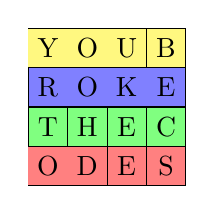
\begin{tikzpicture}[every node/.style={minimum size=.5cm-\pgflinewidth, outer sep=0pt}]
            \draw[step=0.5cm,color=black] (-1,-1) grid (1,1);
            \node[fill=white!50!yellow] at (-0.75,+0.75) {Y};
            \node[fill=white!50!yellow] at (-0.25,+0.75) {O};
            \node[fill=white!50!yellow] at (+0.25,+0.75) {U};
            \node[fill=white!50!yellow] at (+0.75,+0.75) {B};
            \node[fill=white!50!blue] at (-0.75,+0.25) {R};
            \node[fill=white!50!blue] at (-0.25,+0.25) {O};
            \node[fill=white!50!blue] at (+0.25,+0.25) {K};
            \node[fill=white!50!blue] at (+0.75,+0.25) {E};
            \node[fill=white!50!green] at (-0.75,-0.25) {T};
            \node[fill=white!50!green] at (-0.25,-0.25) {H};
            \node[fill=white!50!green] at (+0.25,-0.25) {E};
            \node[fill=white!50!green] at (+0.75,-0.25) {C};
            \node[fill=white!50!red] at (-0.75,-0.75) {O};
            \node[fill=white!50!red] at (-0.25,-0.75) {D};
            \node[fill=white!50!red] at (+0.25,-0.75) {E};
            \node[fill=white!50!red] at (+0.75,-0.75) {S};
        \end{tikzpicture}
    \end{document}
